\section{Accelerometer}\label{section:accelerometer}
Before starting the implementation of the application, the accelerometer of the phone should be examined. 
Knowing the orientation of the accelerometer axis in the phone is important in the implementation of dead reckoning.
As mentioned in \secref{section:limitations}, the phone will be in held in a fixed position when the game is played. 
Which means that sideways movements will be tracked along one axis, and will be used to move the paddle accordingly.
To find the axis orientation, tests have been made by moving the phone in specific directions and looking at the data output. 
The orientation of the accelerometer axis' can be seen in \figref{figure:axis-orientation}.

\begin{figure}[h]
	\centering
	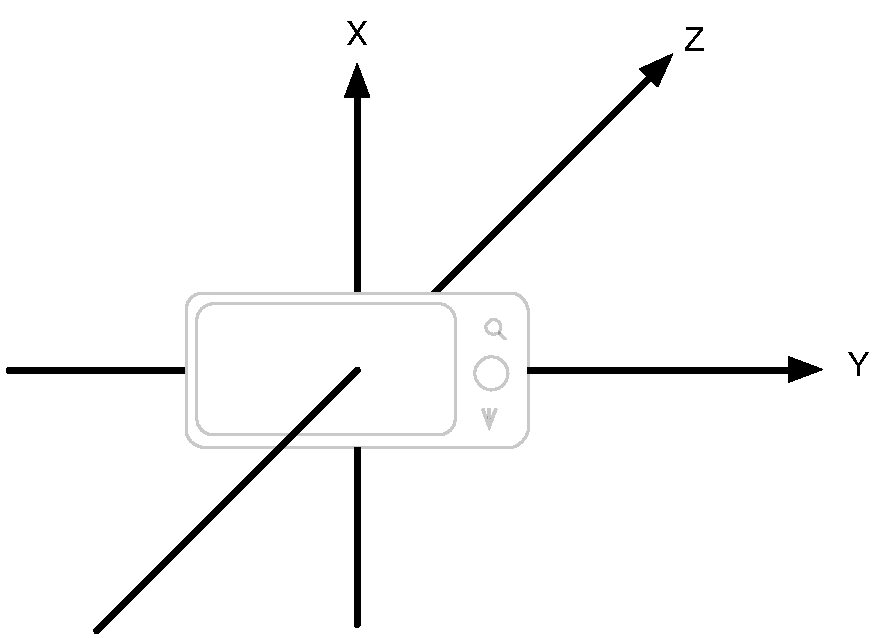
\includegraphics[scale=0.5]{media/phone-rotation/phone-axistocality}
	\caption{The orientation of the accelerometer.}
	\label{figure:axis-orientation}
\end{figure}

Another functionality that needs testing is how the data behaves when the phone is rotated manually around the different axis', which is needed because when the user holds the phone it will be tilted.
In \figref{figure:phone-rotate-y-axis-graph}, a graph shows the accelerations of the axis when the phone is rotated counter-clockwise around the y-axis from the position shown in \figref{figure:axis-orientation}, other recordings was performed for rotation around the other axis' but has been omitted as it does not give new insight to the understanding of the accelerometer.
%pull 90 grader
\begin{figure}[h]
\centering
	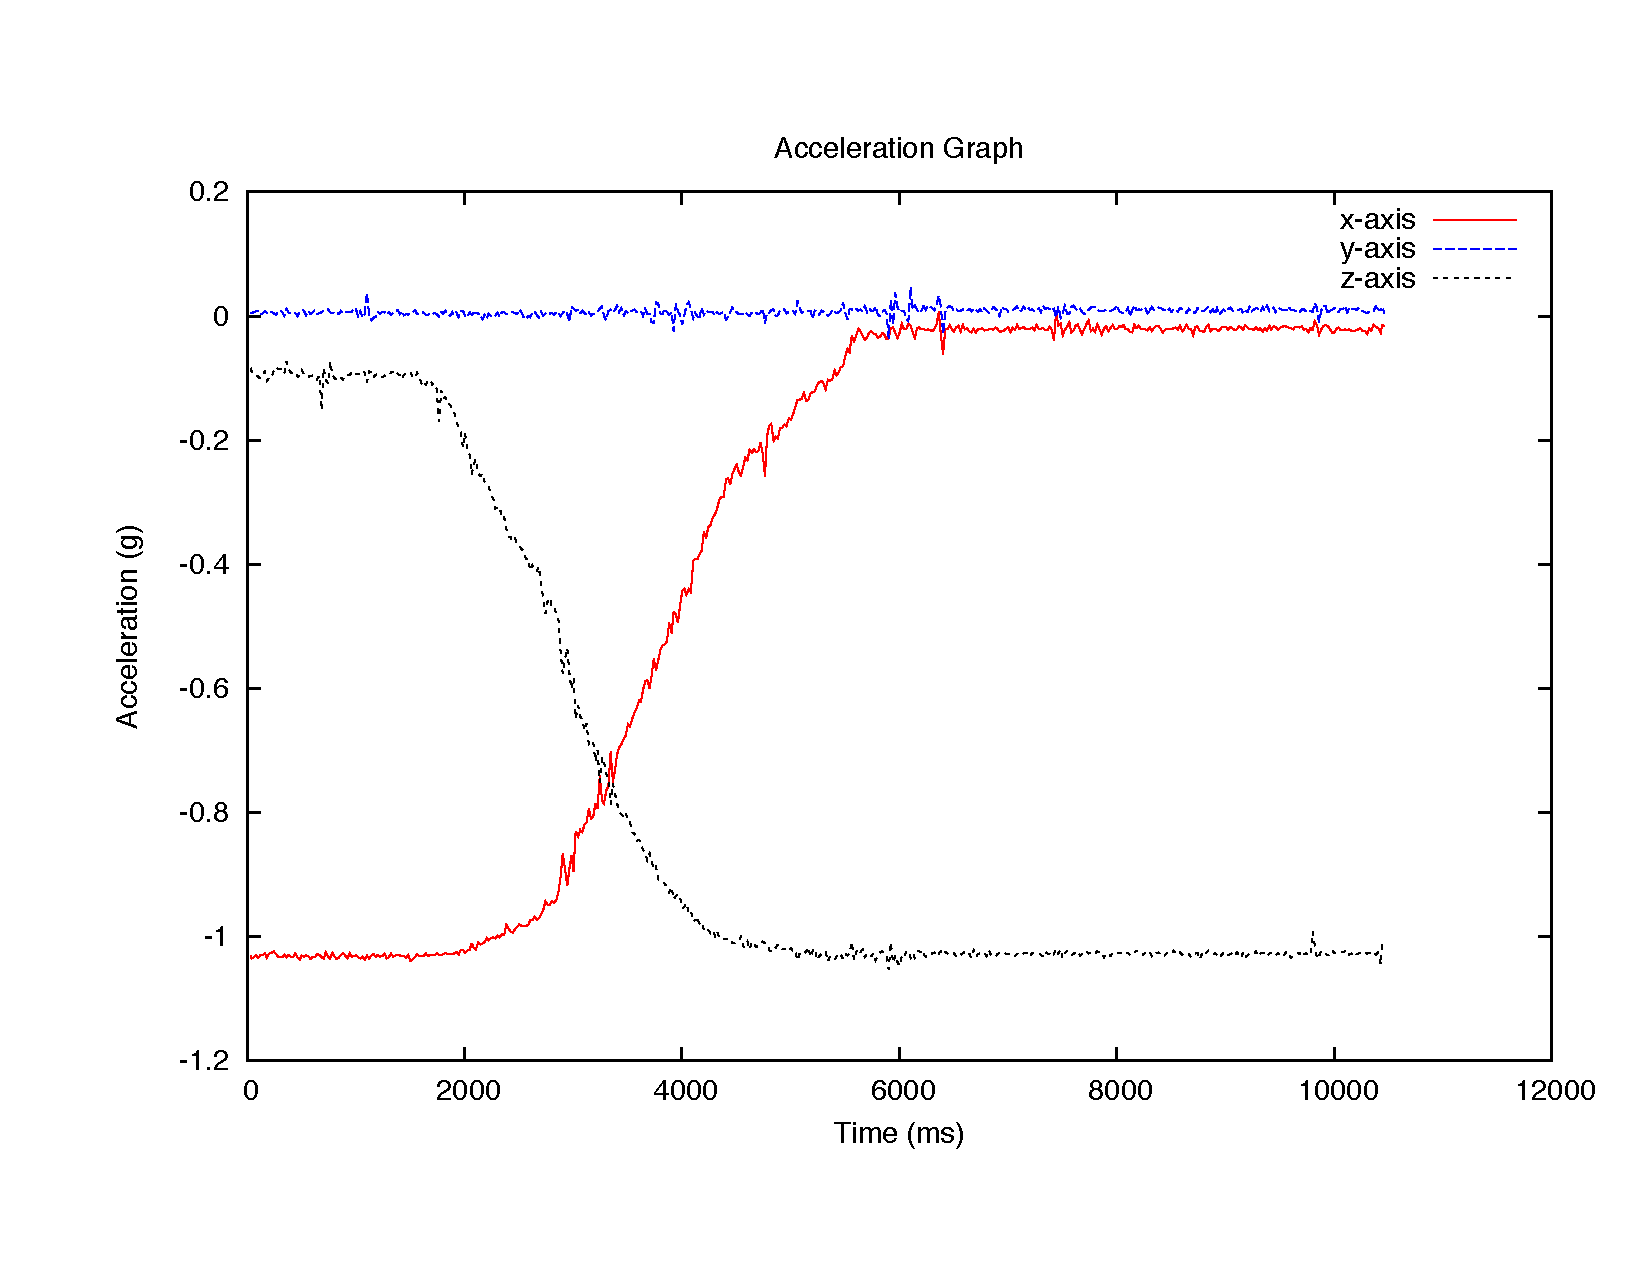
\includegraphics[scale=0.45, trim=0cm 2cm 0cm 2cm]{media/gnuplot/rotation.pdf}
	\caption{Acceleration graph recorded for rotating $90^\circ$ around the y-axis. (Blue = x, Black = y, Green = z)}
	\label{figure:phone-rotate-y-axis-graph}
\end{figure}
When the user is holding the phone as in \figref{figure:axis-orientation}, the accelerations, in the device's y-axis, of a step to the left and to the right can be seen in \figref{figure:step-left-and-right}.
The acceleration is measured in gravitational force (g-force) and the time in milliseconds, where $1 g$ is the gravitational pull.
The accelerometer for the chosen phone have a measurement limit between $-2 g$ and $2 g$.

\begin{figure}[H]
	\centering	
	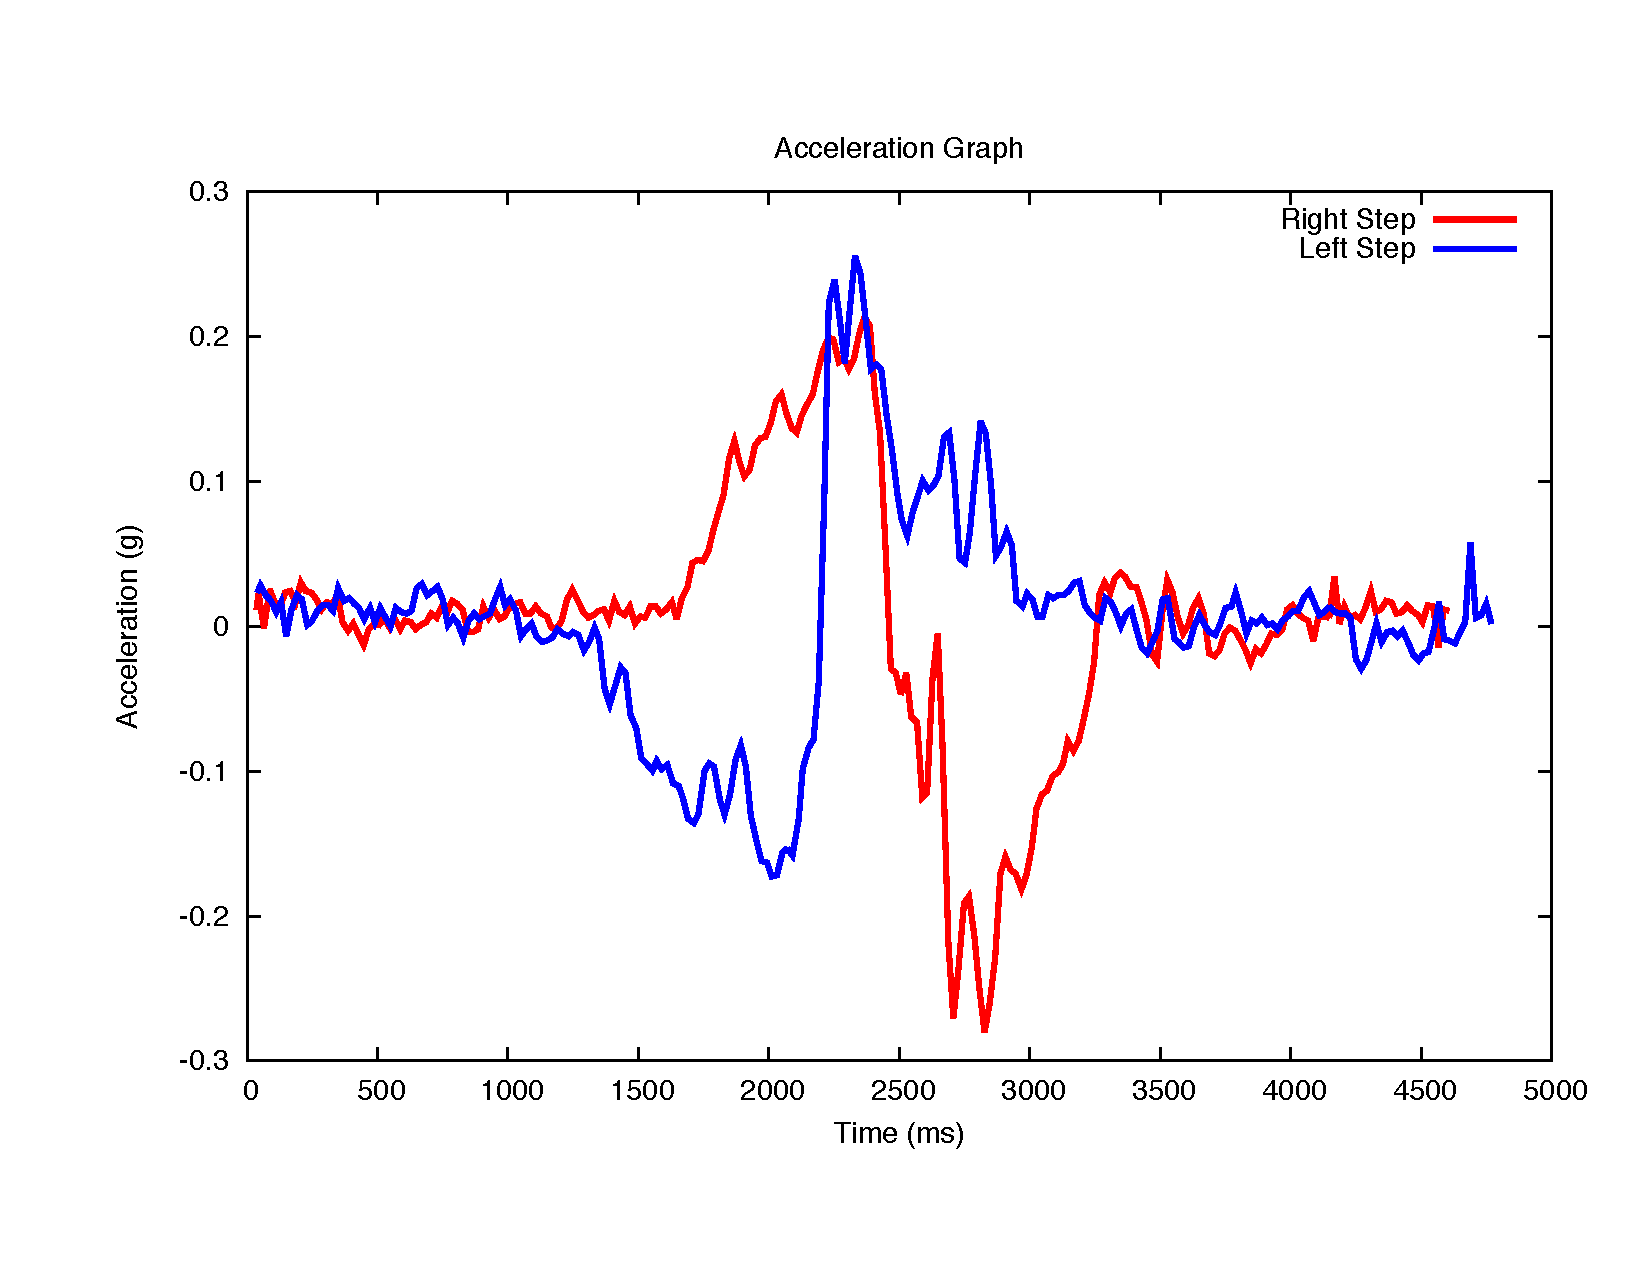
\includegraphics[scale=0.45, trim=0cm 2cm 0cm 2cm]{media/gnuplot/tokew.pdf}
	\caption{A graph showing a left, blue, and a right, red, step.}
	\label{figure:step-left-and-right}
\end{figure}

%Dette billede kan også ses udfra det første billede!
%\begin{figure}
%	\centering
%	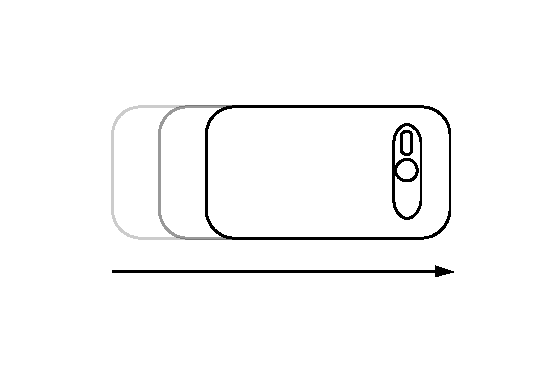
\includegraphics{media/phone-rotation/phone-horizontality}
%	\caption{Phone moving along the y-axis. (Back of the phone)}
%	\label{key}
%\end{figure}


